%introdurre il concetto di varianza per uno stato coerente
\section{Stati coerenti e le loro propriet\`a}\label{se:sezione1-1}
I segnali elettromagnetici possono essere descritti sia attraverso onde che attraverso particelle, ovvero fotoni. Ad esempio, il segnale prodotto da un LASER è ben rappresentato da uno stato quantistico detto stato coerente. Esso comunemente \`e rappresentato $|\alpha_j \rangle = |q_j + ip_j \rangle $ attraverso la notazione introdotta da Paul Dirac che prende il nome di \textit{bra-ket}. Dal punto di vista della fisica classica, il numero complesso $\alpha$ è strettamente legato all'ampiezza di oscillazione del campo elettrico corrispondente al segnale. Esso è costituito da due componenti reali, $q$ e $p$, dette componenti di quadratura. Dal punto di vista della fisica quantistica, tuttavia, non è possibile assegnare un valore preciso a queste grandezze. Infatti, i valori di $q$ e $p$ che utilizziamo per rappresentare lo stato coerente sono solo valori medi. Quando proviamo a fare una misurazione delle grandezze fisiche associate, che indichiamo con $\hat q$ e $\hat p$, esse si comportano come variabili aleatorie che rispondono alla stessa distribuzione di probabilit\`a gaussiana che, in oppurtune unit\`a di misura, ha varianza unitaria. Il motivo per cui non rappresentano un valore esatto \`e perch\'e, a differenza della fisica classica, nella fisica quantistica le quantit\'a, anche scalari, sono degli operatori che assumono una valore esatto solamente in fase di misura.

Ogni stato coerente presenta un numero medio di fotoni che pu\`o essere calcolato nel seguente modo:
\begin{equation}
\langle n_j \rangle = |a_j|^2 = q_j^2 + p_j^2 
\end{equation}

Il numero medio di fotoni di uno stato coerente \`e associato all'energia del segnale di luce che viene inviato, maggiore \`e il numero di fotoni maggiore \`e l'energia del segnale.

Come detto precedentemente, gli stati coerenti si presentano come una distribuzione di probabilit\`a gaussiana e possono essere rappresentati graficamente in un piano cartesiano, che riporta i valori misurabili di $q$ e $p$, come una nuvola di punti i quali avranno appunto probabilit\`a gaussiana di essere estratti.


\begin{figure}[h] 
\begin{center}
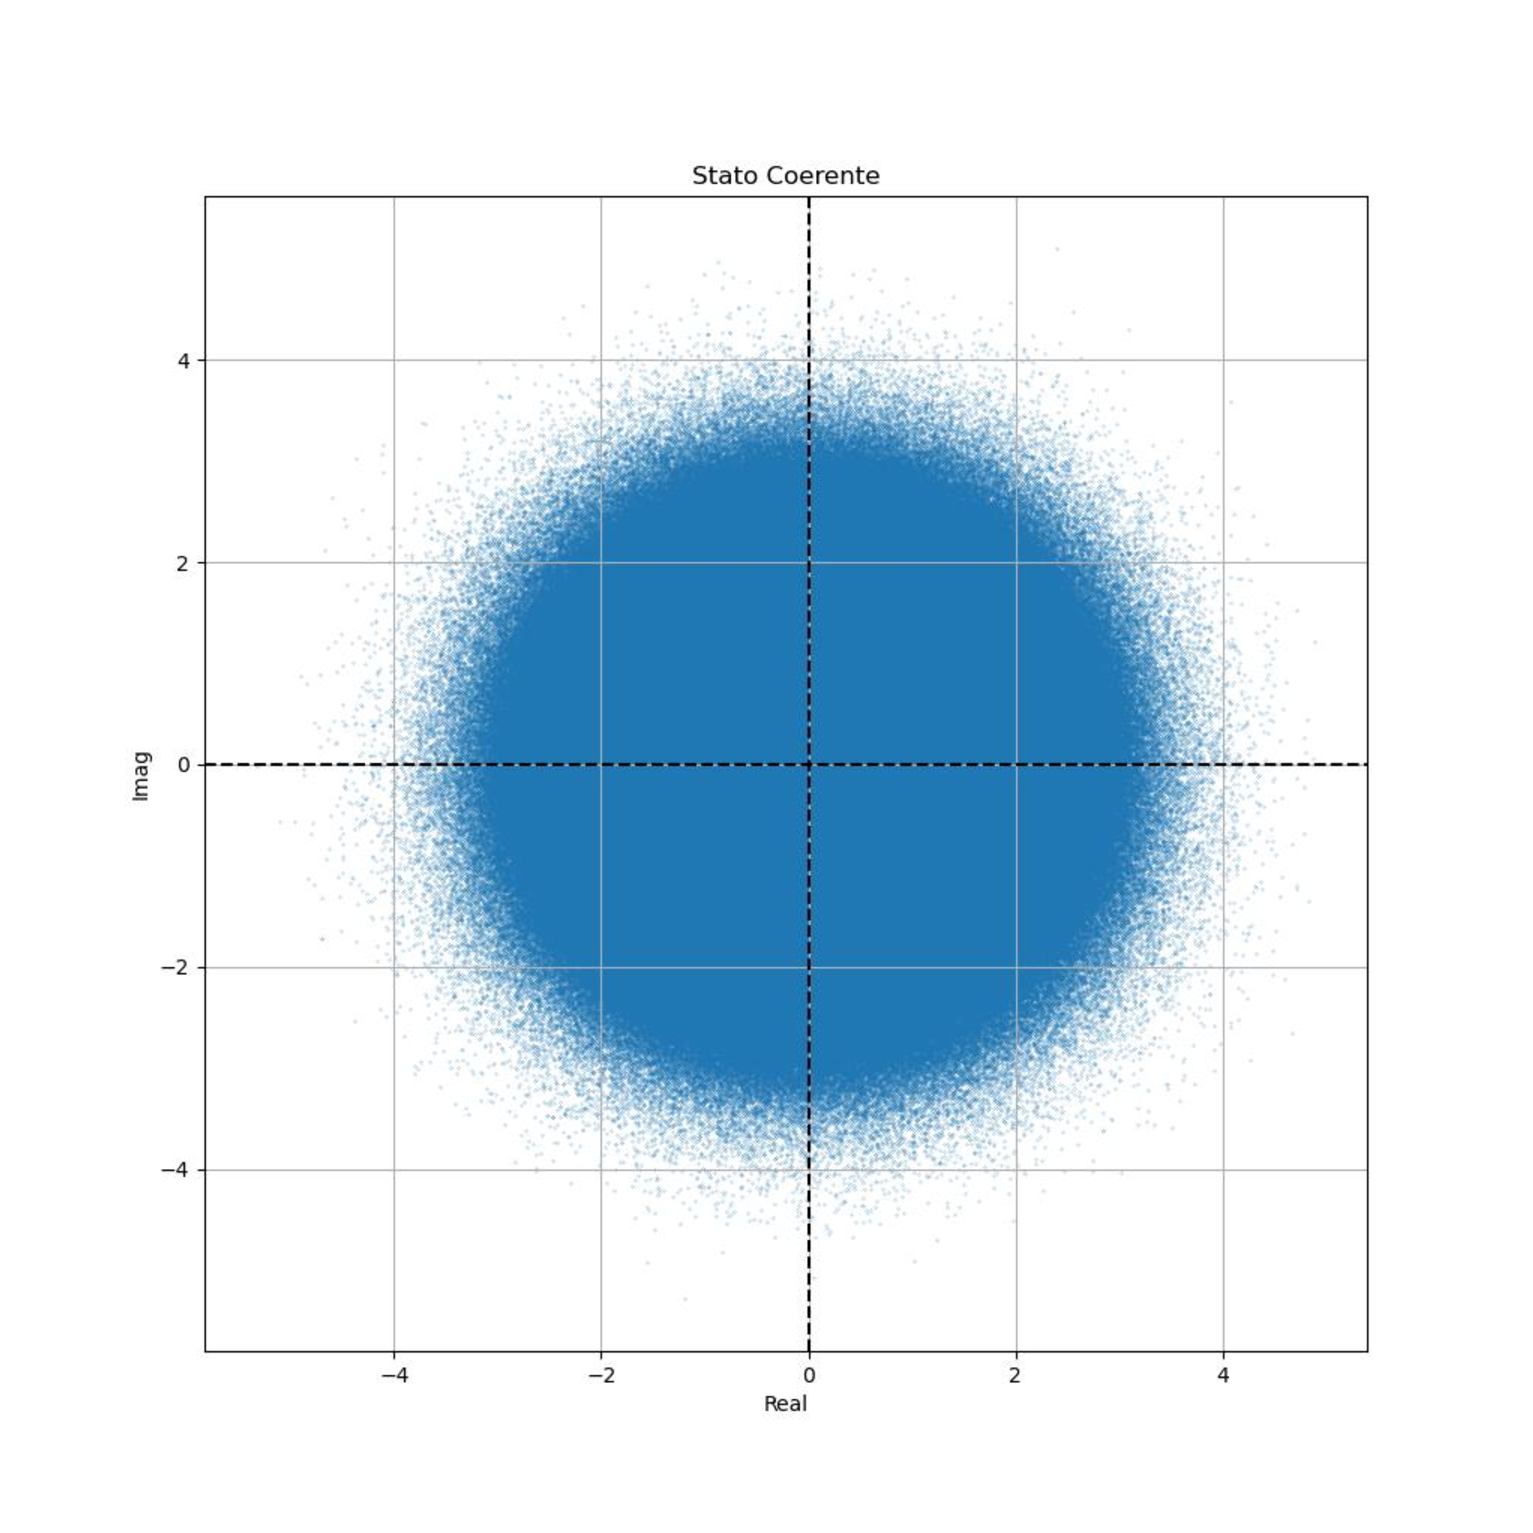
\includegraphics[scale=0.4]{figure/stato_coerente.eps}
\end{center}
\caption[stato-coerente]{Questa figura \`e una gaussiana vista dall'alto che viene ottenuta simulando molte volte la produzione dello stesso stato coerente e la misura della grandezza $\hat q$ o $\hat p$. La gaussiana \`e rappresentata su un piano cartesiano riportante sulle ascisse le misure della componente $q$ mentre sulle ordinate le misure della componente $p$} \label{fig:stato-coerente}
\end{figure}

\section{Misurazione dei segnali e incertezza quantistica}
Partendo dal caso ideale, in cui il canale di comunicazione \`e perfetto e quindi non aggiunge rumore durante la trasmissione, Bob ricever\`a uno stato coerente con la forma vista in figura \ref{fig:stato-coerente} e proverà a misurarlo, con una data incertezza. Da notare che l'incertezza della misura \`e presente anche nel caso di un canale di comunicazione ideale, questo perch\'e non \`e dovuta solamente al rumore esterno, come ci si aspetterebbe in un canale di comunicazione classico, ma \`e una caratteristica intriseca di uno stato quantistico la quale non pu\`o essere rimossa in base al principio di indeterminazione di Heisenberg. Questa incertezza si presenta proprio in fase di misura, perch\'e come detto nella sezione~\ref{se:sezione1-1}, il valore di quadratura $q$ e $p$ sono solamente valori medi mentre il valore $Q$ o $P$ che otteniamo da una misura \ref{subse:sottosezione2-1-1} si comportano come variabili aleatorie con distribuzione di probabilit\`a gaussiana. 

In un trasmissione reale, l'aggiunta di rumore esterno \`e inevitabile e in questo rumore \`e presente anche quello prodotto da un eventuale spia (Eve) che tenta anch'essa di misurare il segnale modificandolo, questo rende la misura di Bob ancora pi\`u incerta come possiamo notare nella figura~\ref{fig:eve-bob}. 

Per concludere possiamo dire che i protocolli di QKD utlizzano due fondamentali caratteristiche dei segnali quantistici:
\begin{itemize}
\item vi è un'incertezza nella misura anche in assenza di rumore esterno;
\item una misura di un segnale introduce rumore nel segnale stesso.
\end{itemize}

%Tali proprietà risultano cruciali per determinare l'eventuale intromissione di Eve nella comunicazione e quindi la possibilit\`a o meno di creare una chiave crittografica sicura.
Tali proprietà risultano cruciali per determinare l'eventuale intromissione di Eve nella comunicazione e per nascondere i bit trasmessi da Eve.

\begin{figure}[tbp] 
\begin{center}
\begin{tabular}{c @{\hspace{1em}} c}
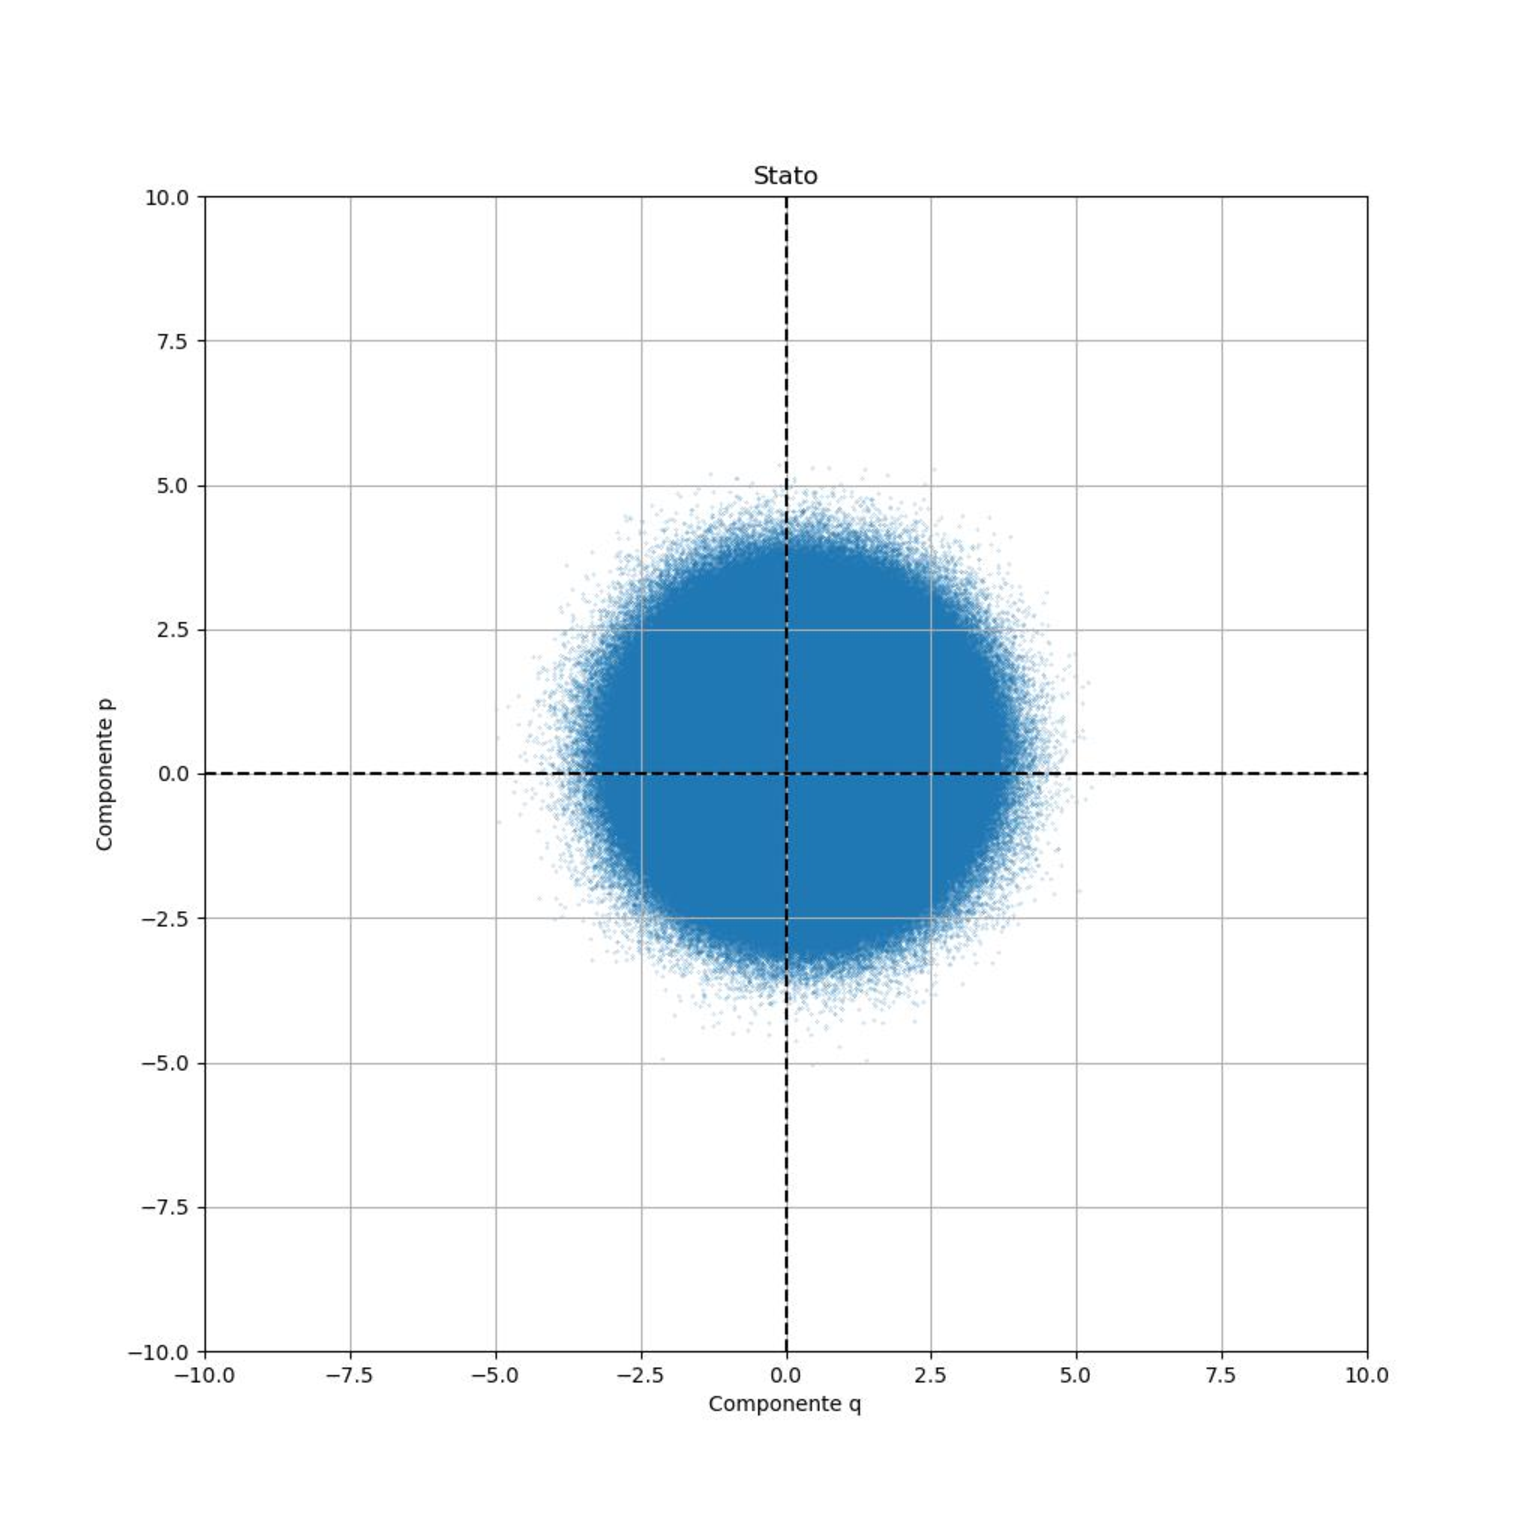
\includegraphics[width=7cm]{figure/stato-bob.eps} &
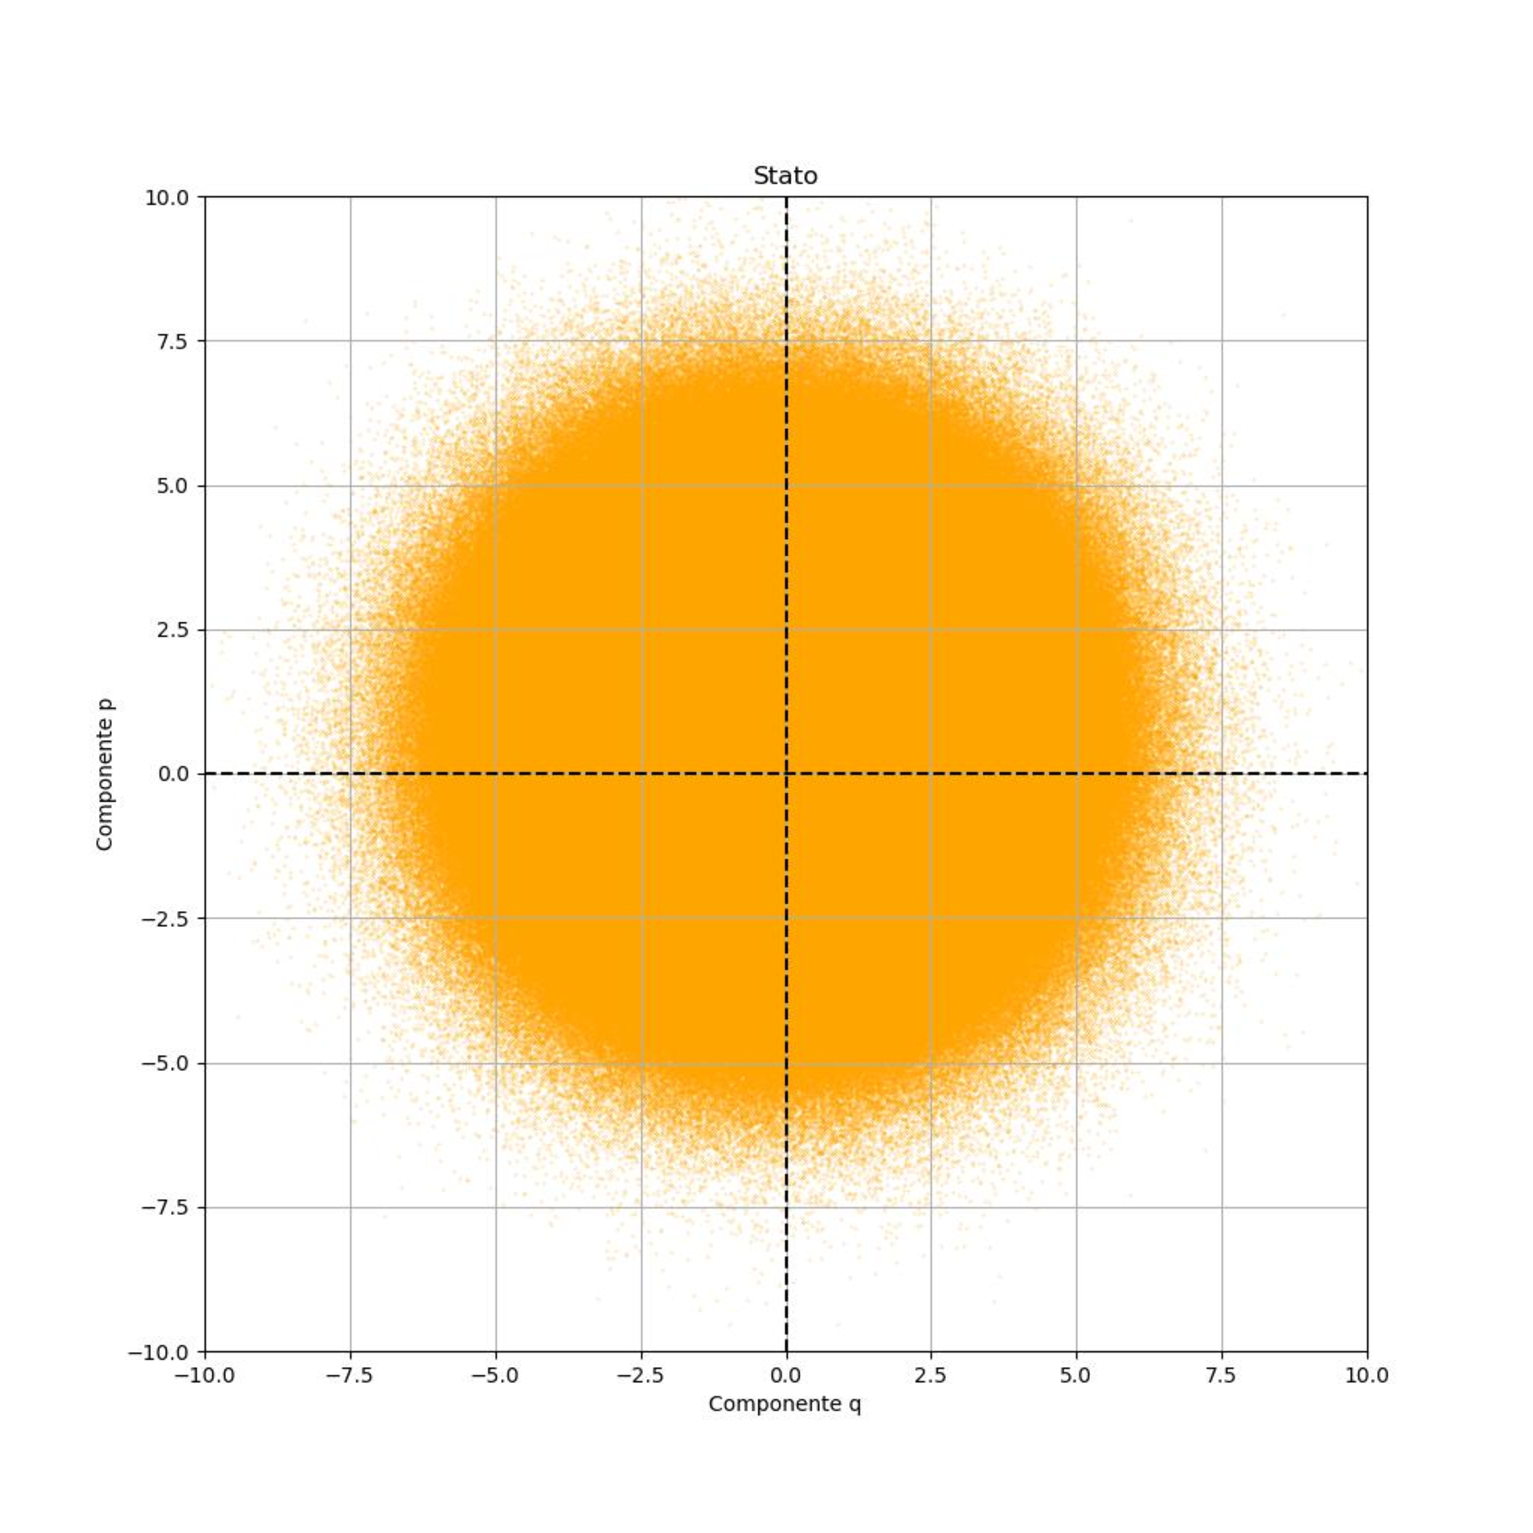
\includegraphics[width=7cm]{figure/stato-eve.eps} \\
 (a) & (b)
\end{tabular}
\end{center}
\caption[Confronto stato con spia e senza]{Esempio di rappresentazione dello stesso stato: (a) lo stato non \`e stato alterato da Eve; (b) Eve ha misurato lo stato per poi re-inviarlo a Bob  } \label{fig:eve-bob}
\end{figure}
